\documentclass[tikz,border=7pt]{standalone}
\usepackage{amsmath,pgfplots}
\pgfplotsset{compat=1.18}
\definecolor{ink}{HTML}{21352F}\definecolor{teal}{HTML}{087F7B}
\definecolor{gold}{HTML}{C58B2A}\definecolor{blue}{HTML}{4B77A8}\definecolor{rose}{HTML}{B65A62}
\begin{document}
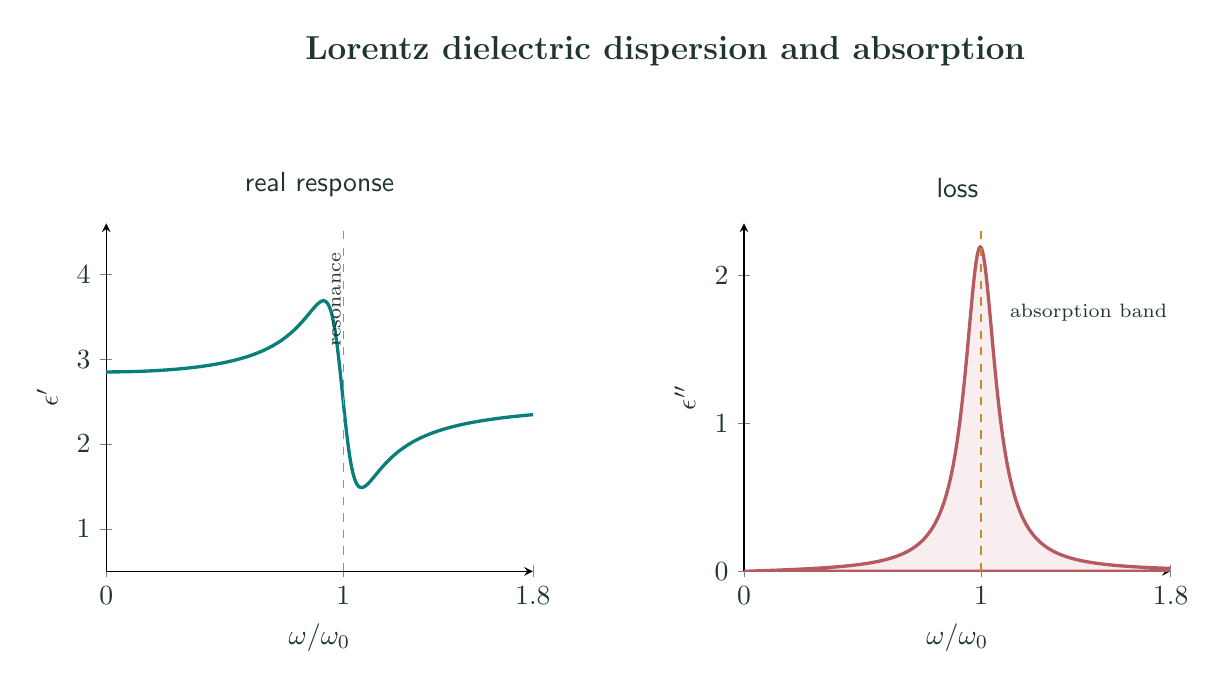
\begin{tikzpicture}[font=\sffamily,text=ink]
\node[font=\bfseries\large] at (0,3.8) {Lorentz dielectric dispersion and absorption};
\begin{axis}[at={(-7.1cm,-2.8cm)},anchor=south west,width=7cm,height=6cm,xmin=0,xmax=1.8,ymin=.5,ymax=4.6,
 axis lines=left,xlabel={$\omega/\omega_0$},ylabel={$\epsilon'$},xtick={0,1,1.8},title={real response}]
 \addplot[teal,very thick,domain=0:1.8,samples=420]{2.5+.35*(1-x^2)/((1-x^2)^2+.0256*x^2)};
 \draw[gold,dashed] (axis cs:1,.5)--(axis cs:1,4.6);
 \node[font=\scriptsize,rotate=90,anchor=south] at (axis cs:1.03,3.7) {resonance};
\end{axis}
\begin{axis}[at={(1.0cm,-2.8cm)},anchor=south west,width=7cm,height=6cm,xmin=0,xmax=1.8,ymin=0,ymax=2.35,
 axis lines=left,xlabel={$\omega/\omega_0$},ylabel={$\epsilon''$},xtick={0,1,1.8},title={loss}]
 \addplot[rose,very thick,domain=0:1.8,samples=420,fill=rose!10]{.35*.16*x/((1-x^2)^2+.0256*x^2)}\closedcycle;
 \draw[gold,dashed] (axis cs:1,0)--(axis cs:1,2.35);
 \node[font=\scriptsize,anchor=west] at (axis cs:1.08,1.75) {absorption band};
\end{axis}
\end{tikzpicture}
\end{document}
